\documentclass[../analisi-dei-requisiti.tex]{subfiles}

\begin{document}

\subsection{Attori}
\label{subs:attori}

\subsubsection{Attori primari}
\label{sssec:attori_primari}
\begin{description}
  \item[Utente generico:] È l'utilizzatore del prodotto, una persona autenticata e interessata ad interagire con Grafana per visualizzare le previsioni e/o le zone di criticità individuate dal plug-in;
  \item[Utente amministratore:] È l'utente autenticato nel sistema nel ruolo di amministratore, che oltre ad avere la possibilità di intereagire con Grafana, gestisce il programma di addestramento per i modelli di machine learning e gestisce la configurazione del plug-in sul flusso di dati monitorati da Grafana.
\end{description}

\subsubsection{Attori secondari}
\label{sssec:attori_secondari}
\begin{description}
  \item[Grafana:] Piattaforma che permette di essere estesa con dei plug-in, in essa infatti risiederà il nostro prodotto che permetterà all'utente di visualizzare le previsioni ottenute dal plug-in sviluppato dal team.
\end{description}

\subsection{Elenco dei casi d'uso}
\label{subs:elenco_dei_casi_duso}

\subsubsection{UC1 - Addestramento del sistema}
\label{sssec:uc1}

\begin{description}
  \item[Attore primario:] Utente amministratore.
  \item[Descrizione:] Per creare il file JSON contenente il predittore da dare al sistema di monitoraggio Grafana l'amministratore deve creare un file contenente i dati, scegliere il modello di machine learning da utilizzare e infine deve avviare l'addestramento.
  \item[Precondizione:] L'amministratore deve avere dei dati e sapere che modello utilizzare.
  \item[Scenario principale:]
  \begin{enumerate}
    \item L'amministratore inserisce i dati (UC1.1);
    \item L'amministratore utilizza un predittore già addestrato, se ne è in possesso (UC1.2);
    \item L'amministratore sceglie il modello di machine learning (UC1.3);
    \item L'amministratore avvia l'addestramento (UC1.4);
    \item L'amministratore crea un file contenente il predittore (UC1.5).
  \end{enumerate}
  \item[Postcondizione:] Si è ottenuto un file contente il predittore da dare a Grafana.
\end{description}

\subsubsection{UC1.1 - Inserimento dati di allenamento}
\label{sssec:uc1.1}
\begin{description}
  \item[Attore primario:] Utente amministratore.
  \item[Descrizione:] L'amministratore inserisce i dati raccolti da un database in un file CSV.
  \item[Precondizione:] L'amministratore è in possesso di dati.
  \item[Scenario principale:]
  \begin{enumerate}
    \item L'amministratore caricati i dati all'interno del file CSV;
    \item I dati vengono caricati nel sistema.
  \end{enumerate}
  \item[Postcondizione:] Il file CSV contiene i dati raccolti dall'amministratore.
\end{description}

\subsubsection{UC1.2 - Utilizzo del predittore già addestrato}
\label{sssec:uc1.2}
\begin{description}
  \item[Attore primario:] Utente amministratore.
  \item[Descrizione:] L'amministratore utilizza il file JSON contenente il predittore addestrato in un'applicazione esterna.
  \item[Precondizione:] L'amministratore ha a disposizione il predittore già allenato.
  \item[Scenario principale:] L'amministratore, qualora possieda un predittore precedentemente allenato, lo carica nel sistema.
  \item[Postcondizione:] L'amministratore ha a disposizione un predittore già addestrato.
\end{description}

\subsubsection{UC1.3 - Scelta del modello di machine learning}
\label{sssec:uc1.3}
\begin{description}
  \item[Attore primario:] Utente amministratore.
  \item[Descrizione:] L'amministratore decide che tipo di machine learning utilizzare: SVM, RL o la Rete Neurale.
  \item[Precondizione:]
  \begin{enumerate}
    \item L'inserimento dei dati è avvenuto correttamente (UC1);
    \item L'amministratore ha a disposizione i tre modelli di machine learning.
  \end{enumerate}
  \item[Scenario principale:] L'amministratore, avente un file contenente i dati, decide che modello di machine learning utilizzare tra SVM, RL o la Rete Neurale.
  \item[Postcondizione:] L'amministratore ha scelto un modello di machine learning.
\end{description}

\subsubsection{UC1.3.1 - Scelto modello Support Vector Machine}
\label{sssec:uc1.3.1}
\begin{description}
  \item[Attore primario]: Utente amministratore.
  \item[Descrizione]: L'amministratore ha scelto come modello la Support Vector Machine.
  \item[Precondizione:]
  \begin{enumerate}
    \item L'inserimento dei dati è avvenuto correttamente (UC1);
    \item L'amministratore ha a disposizione i tre modelli di machine learning.
  \end{enumerate}
  \item[Scenario principale:] L'amministratore ha selezionato SVM come algoritmo per svolgere l'addestramento.
  \item[Postcondizione]: L'amministratore ha scelto come modello la SVM.
\end{description}

\subsubsection{UC1.3.2 - Scelto modello Regressione Lineare}
\label{sssec:uc1.3.2}
\begin{description}
  \item[Attore primario]: Utente amministratore.
  \item[Descrizione]: L'amministratore ha scelto come modello la Regressione Lineare.
  \item[Precondizione:]
  \begin{enumerate}
    \item L'inserimento dei dati è avvenuto correttamente (UC1);
    \item L'amministratore ha a disposizione i tre modelli di machine learning.
  \end{enumerate}
  \item[Scenario principale:] L'amministratore ha selezionato la RL come algoritmo per svolgere l'addestramento.
  \item[Postcondizione]: L'amministratore ha scelto come dello la RL.
\end{description}

\subsubsection{UC1.3.2.1 - Scelto modello Regressione Esponenziale}
\label{sssec:uc1.3.2.1}
\begin{description}
  \item[Attore primario]: Utente amministratore.
  \item[Descrizione]: L'amministratore ha scelto come modello la Regressione Esponenziale.
  \item[Precondizione:]
  \begin{enumerate}
    \item L'inserimento dei dati è avvenuto correttamente (UC1);
    \item L'amministratore ha a disposizione i tre modelli di machine learning.
  \end{enumerate}
  \item[Scenario principale:] L'amministratore ha selezionato la Regressione Esponenziale come algoritmo per svolgere l'addestramento.
  \item[Postcondizione]: L'amministratore ha scelto come modello la Regressione Esponenziale.
\end{description}

\subsubsection{UC1.3.2.2 - Scelto modello Regressione Logaritmica}
\label{sssec:uc1.3.2.2}
\begin{description}
  \item[Attore primario]: Utente amministratore.
  \item[Descrizione]: L'amministratore ha scelto come modello la Regressione Logaritmica.
  \item[Precondizione:]
  \begin{enumerate}
    \item L'inserimento dei dati è avvenuto correttamente (UC1);
    \item L'amministratore ha a disposizione i tre modelli di machine learning.
  \end{enumerate}
  \item[Scenario principale:] L'amministratore ha selezionato la Regressione Logaritmica come algoritmo per svolgere l'addestramento.
  \item[Postcondizione]: L'amministratore ha scelto come modello la Regressione Logaritmica.
\end{description}

\subsubsection{UC1.3.3 - Scelto modello Rete Neurale}
\label{sssec:uc1.3.3}
\begin{description}
  \item[Attore primario]: Utente amministratore.
  \item[Descrizione]: L'amministratore ha scelto come modello la Rete Neurale;
  \item[Precondizione:]
  \begin{enumerate}
    \item L'inserimento dei dati è avvenuto correttamente (UC1);
    \item L'amministratore ha a disposizione i tre modelli di machine learning.
  \end{enumerate}
  \item[Scenario principale:] L'amministratore ha selezionato la Rete Neurale come algoritmo per svolgere l'addestramento.
  \item[Postcondizione]: L'amministratore ha scelto come modello la Rete Neurale.
\end{description}


\subsubsection{UC1.4 - Avvio dell'addestramento}
\label{sssec:uc1.4}
\begin{description}
  \item[Attore primario:] Utente amministratore.
  \item[Descrizione:] L'amministratore utilizzando la libreria e i dati ottiene il predittore.
  \item[Precondizione:]
  \begin{enumerate}
    \item L'amministratore ha a disposizione il file contenente i dati (UC1);
    \item L'amministratore ha scelto un modello di machine learning.
  \end{enumerate}
  \item[Scenario principale:] Avendo a disposizione il file con i dati e avendo scelto un modello avviene l'addestramento.
  \item[Postcondizione:] Si è ottenuto il predittore.
\end{description}

\subsubsection{UC1.5 - Salvataggio del risultati ottenuti}
\label{sssec:uc1.5}
\begin{description}
  \item[Attore primario:] Utente amministratore.
  \item[Descrizione:] I risultati ottenuti vengono salvati nel file JSON, riportando anche la tipologia di modello di machine learning utilizzato.
  \item[Precondizione:]
  \begin{enumerate}
    \item L'amministratore ha i dati ottenuti in precedenza;
    \item L'amministratore ha deciso che modello di machine learnig  utilizzare.
  \end{enumerate}
  \item[Scenario principale:] Una volta ottenuti i risultati dall'addestramento, l'amministratore salva i dati e il modello utilizzato nel file JSON.
  \item[Postcondizione:] Il file contiene sia il predittore che il modello utilizzato.
\end{description}


\newpage
\subsubsection{UC2 - Addestramento del predittore}
\label{sssec:uc2}

\begin{figure}[h!]
  \begin{center}
    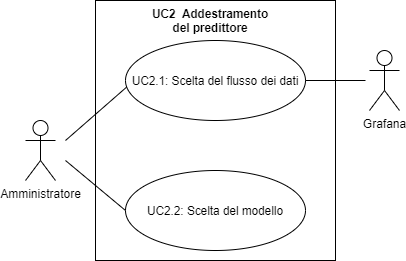
\includegraphics[width=19cm]{uc2.png}\\
    \caption{UC2 - Addestramento del predittore}%
    \label{fig:uc2}
  \end{center}
\end{figure}

\begin{itemize}
  \item \textbf{Attore primario}:  Utente;
  \item \textbf{Attore secondario}: Grafana;
  \item \textbf{Descrizione}: L'utente seleziona un flusso di dati presente in Grafana e il plug-in, grazie allo storico dei dati di quel flusso, addestara il predittore utilizzando un modello;
  \item \textbf{Precondizione}: L'utente ha creato un pannello del plug-in e sa che tipo di modello di machine learning va utilizzato;
  \item \textbf{Scenario principale}:
  \begin{enumerate}
    \item L'utente sceglie su che dati, tra quelli disponibili in Grafana, compiere l'addestramento (UC2.1);
    \item L'utente sceglie un modello da utlizzare per compiere l'addestramento(UC2.2).
  \end{enumerate}
  \item \textbf{Postcondizione}: Il plug-in ha generato il predittore ed ora è pronto a fare previsioni sui dati.
\end{itemize}

\paragraph{UC2.1 - Scelta del flusso dei dati}
\label{para:uc2.1}
\begin{itemize}
  \item \textbf{Attore primario}: Utente;
  \item \textbf{Attore secondario}: Grafana;
  \item \textbf{Descrizione}: L'utente sceglie su che flusso presente in Grafana compiere l'addestramento;
  \item \textbf{Precondizione}: L'utente ha a disposizione dei dati;
  \item \textbf{Scenario principale}: L'attore sceglie il flusso di dati per effettuare l'addestramento;
  \item \textbf{Postcondizione}: L'utente ha scelto un flusso di dati e con questo farà l'addestramento.
\end{itemize}

\paragraph{UC2.2 - Scelta del modello}
\label{para:uc2.2}
\begin{itemize}
  \item \textbf{Attore primario}: Utente;
  \item \textbf{Descrizione}: L'utente sceglie un modello da applicare ai dati tra SVM, RL, regressione esponenziale, regressione logaritmica, SVM adattata alla regressione o rete neurale;
  \item \textbf{Precondizione}:
  \item \begin{enumerate}
    \item L'utente ha scelto su che dati, tra quelli disponibili in Grafana, compiere l'addestramento (UC2.1);
    \item L'utente deve scegliere che modello di machine laerning utilizzare.
  \end{enumerate}
  \item \textbf{Scenario principale}: L'utente sceglie il modello da utilizzare per l'addestramento;
  \item \textbf{Postcondizione}: L'utente ha scelto il modello per l'addestramento;
  \item \textbf{Generalizzazioni}: UC2.2 viene generalizzato dai casi d'uso UC6, UC7, UC8, UC9, UC10 e UC11.
\end{itemize}



\newpage
\subsubsection{UC3 - Configurazione del plug-in}
\label{sssec:uc3}

\begin{figure}[h!]
  \begin{center}
    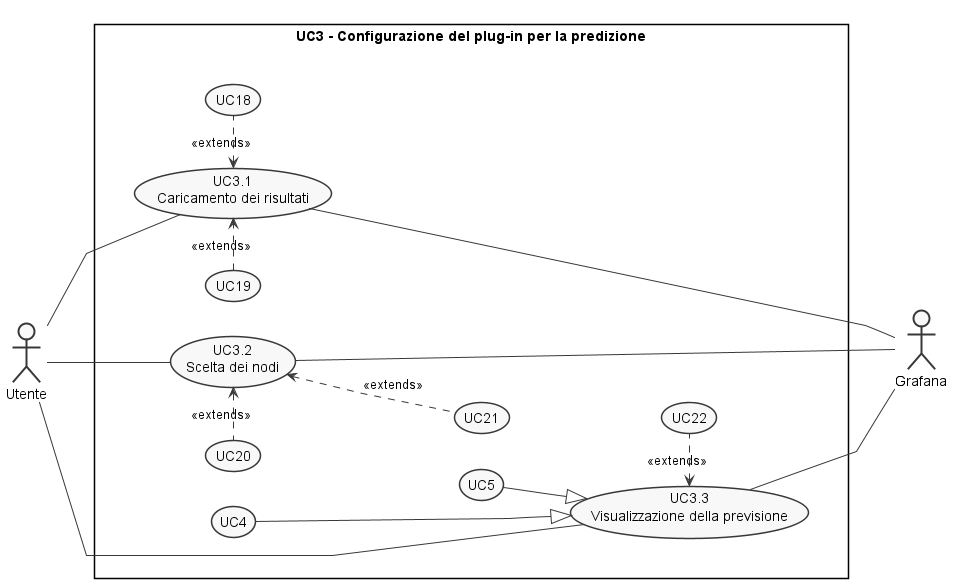
\includegraphics[width=12cm]{uc3.png}\\
    \caption{UC3 - Configurazione del plug-in}%
    \label{fig:uc3}
  \end{center}
  \end{figure}

\begin{description}
  \item[Attore primario]: Utente amministratore.
  \item[Attore secondario]: Grafana.
  \item[Descrizione:] Configurazione del plug-in per ottenere delle previsioni.
  \item[Precondizione:] L'amministratore ha abilitato il plug-in e si trova nella pagina di configurazione.
  \item[Scenario principale:]
  \begin{enumerate}
    \item L'amministratore carica il file JSON contente i risultati dell'addestramento (UC3.1);
    \item L'amministratore sceglie su quali nodi fare le previsioni (UC3.2);
    \item L'amministratore scegli con quale modalità visualizzare i dati (UC3.3).
  \end{enumerate}
  \item[Postcondizione:] L'amministratore ha configurato il plug-in, il quale diventa pronto per essere avviato.
\end{description}

\paragraph{UC3.1 - Caricamento risultati}
\label{sssec:uc3.1}
\begin{description}
  \item[Attore primario:] Utente amministratore.
  \item[Descrizione:] L'amministratore carica il file JSON contenente i risultati ottenuti dall'addestramento.
  \item[Precondizione:] L'amministratore ha a disposizione un file con all'interno i risultati (UC1.5).
  \item[Scenario principale:] L'amministratore carica il file JSON contenente i risultati ottenuti dall'addestramento.
  \item[Postcondizione:] L'amministratore ha caricato il file contenente i risultati dell'addestramento avvenuto precedentemente.
  \item[Estensioni:]
  \begin{enumerate}
	\item UC3.1 viene esteso nel caso d'uso UC9 con la visualizzazione del messaggio di errore quando viene fornito un predittore in un formato non valido;
	\item UC3.1 viene esteso nel caso d'uso UC10 con la visualizzazione del messaggio di errore quando l'amministratore non inserisca alcun file per l'addestramento.
  \end{enumerate}
\end{description}

\paragraph{UC3.2 - Scelta dei nodi}
\label{sssec:uc3.2}
\begin{description}
  \item[Attore primario:] Utente amministratore.
  \item[Descrizione:] L'amministratore sceglie su che nodi effettuare la previsione.
  \item[Precondizione:] L'amministratore ha il file di dati di addestramento (UC3.1).
  \item[Scenario principale:] L'amministratore, data una lista di nodi, seleziona quali vuole aggiungere alla predizione.
  \item[Postcondizione:] L'amministratore ha selezionato i nodi da aggiungere alla predizione.
  \item[Estensioni:]
  \begin{enumerate}
	\item UC3.1 viene esteso nel caso d'uso UC11 con la visualizzazione del messaggio di errore quando non viene selezionato nessun nodo valido;
	\item UC3.1 viene esteso nel caso d'uso UC12 con la visualizzazione del messaggio di errore quando non viene selezionato alcun nodo.
  \end{enumerate}
\end{description}

\paragraph{UC3.3 - Scelta della modalità di visualizzazione}%
\label{sssec:uc3.3}

\begin{figure}[h!]
  \begin{center}
    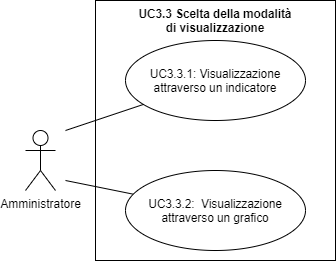
\includegraphics[width=10cm]{uc3.3.png}\\
    \caption{UC3.3 - Scelta della modalità di visualizzazione}%
    \label{fig:uc3.3}
  \end{center}
\end{figure}

\begin{description}
  \item[Attore primario:] Utente amministratore.
  \item[Descrizione:] L'amministratore seleziona il tipo di visualizzazione.
  \item[Precondizione:]  L'amministratore ha selezionato i nodi da utlizzare per la previsione (UC3.2).
  \item[Scenario principale:] L'amministratore sceglie se visualizzare i dati generati dalla previsione per mezzo di un indicatore o di un grafico.
  \item[Postcondizione:] L'amministratore ha scelto che modalità di visualizzazione usare.
  \item[Estensioni:] UC3.3 viene esteso nel caso d'uso UC13 con la visualizzazione del messaggiore di errore quando non viene scelta una modalità di visualizzazione.
\end{description}

\subparagraph{UC3.3.1 - Visualizzazione attraverso un indicatore}
\label{sssec:uc3.3.1}
\begin{description}
  \item[Attore primario:] Utente amministratore.
  \item[Descrizione:] L'indicatore viene scelto come modalità di visualizzazione dei dati.
  \item[Precondizione:] L'amministratore ha a disposizione le due modalità.
  \item[Scenario principale:] L'amministratore sceglie l'indicatore per visualizzare i dati generati dalla previsione.
  \item[Postcondizione:] L'amministratore ha deciso di utilizzare l'indicatore.
\end{description}

\subparagraph{UC3.3.2 - Visualizzazione attraverso un grafico}
\label{sssec:uc3.3.2}
\begin{description}
  \item[Attore primario:] Utente amministratore.
  \item[Descrizione:] Il grafico viene scelto come modalità di visualizzazione dei dati.
  \item[Precondizione:] L'amministratore ha a disposizione le due modalità.
  \item[Scenario principale:] L'amministratore sceglie il grafico per visualizzare i dati generati dalla previsione.
  \item[Postcondizione:] L'amministratore ha deciso di utilizzare il grafico.
\end{description}


\subsubsection{UC4 - Visualizzazione attraverso un grafico}
\label{sssec:uc4}
\begin{itemize}
  \item \textbf{Attore primario}: Utente;
  \item \textbf{Descrizione}: L'attore sceglie di visualizzare la previsione attraverso un diagramma cartesiano;
  \item \textbf{Precondizione}: L'utente deve scegliere il modo per visualizzare la previsione;
  \item \textbf{Scenario principale}: L'utente decide di visualizzare la previsione ottenuta attraverso un grafico, che rappresenta i valori per mezzo di un diagramma cartesiano;
  \item \textbf{Postcondizione}: L'utente ha selezionato il grafico come modalità per visualizzare la previsione.
\end{itemize}


\subsubsection{UC5 - Configurazione alert}
\label{sssec:uc5}
\begin{description}
	\item[Attore primario:] Utente amministratore.
	\item[Attore secondario:] Grafana.
	\item[Descrizione:] L'amministratore imposta degli alert con delle soglie di massima utilizzando i meccanismi offerti da Grafana.
	\item[Precondizione:] 
	\begin{enumerate}
		\item L'amministratore ha configurato il plug-in correttamente(UC4);
		\item L'amministratore avvia il plug-in (UC4.1).
	\end {enumerate}
	\item[Scenario Principale:] L'amministratore definisce l'alert usando l'opzione "Crea alert"(UC5.1) che permette di definire una soglia per l'alert appena creato(UC5.2) tutto ciò usando i meccanismi offerti da Grafana.
	\item[Postcondizione:] L'amministratore ha impostato correttamente le soglie dei alert aggiunti tramite Grafana.
\end{description}

\subsubsection{UC5.1 - Creazione alert}
\label{sssec:uc5.1}
\begin{description}
	\item[Attore primario:] Utente amministratore.
	\item[Attore secondario:] Grafana.
	\item[Precondizione:] L'amministratore si trova sul pannello di predizione.
	\item[Scenario Principale:] L'amministratore aggiunge un alert tramite l'opzione "Crea alert".
	\item[Postcondizione:] L'amministratore visualizza la pagina delle impostazione del pannello con la possibilità di aggiungere alert definiti da Grafana.
\end{description}

\subsubsection{UC5.2 - Definizione soglia massimale}
\label{sssec:uc5.2}
\begin{description}
	\item[Attore primario:] Utente amministratore.
	\item[Attore secondario:] Grafana.
	\item[Precondizione:] L'amministratore ha selezionato l'opzione di inserimento di una soglia tramite l'opzione "Crea alert"(UC5.1).
	\item[Scenario Principale:] L'amministratore tramite Grafana definisce la soglia per l'alert e invia la conferma della creazione del suddetto.
	\item[Postcondizione:] L'amministratore ha impostato la soglia tale che parte l'alert impostato tramite Grafana.
\end{description}

\subsubsection{UC6 - Rimozione del pannello selezionato}
\label{sssec:uc6}
\begin{description}
	\item[Attore primario:] Utente amministratore.
	\item[Attore secondario:] Grafana.
	\item[Descrizione:] L'amministratore seleziona il pannello che vuole rimuovere usando i meccanismi di Grafana.
	\item[Precondizione:]
	\begin{enumerate}
		\item L'amministratore deve aver impostato correttamente il pannello di monitoraggio(UC3.1);
		\item L'amministratore deve aver avviato correttamente il plug-in(UC4.1).
	\end{enumerate}
	\item[Scenario Principale:] L'amministratore seleziona il pannello di monitoraggio da eliminare ed usando le impostazioni di Grafana lo rimuove.
	\item[Postcondizione:] L'amministratore rimuove il pannello di monitoraggio selezionato.
	\item[Estensioni:] UC6 viene esteso nel caso d'uso UC15 con la visualizzazione del messaggio di errore quando si tenta di rimuovere un pannello senza che venga interrotta la predizione.
\end{description}


\subsubsection{UC7 - Scelto modello regressione lineare}%
\label{sssec:uc7}
\begin{itemize}
  \item \textbf{Attore primario}: Utente;
  \item \textbf{Descrizione}: L'utente ha scelto come modello la regressione lineare;
  \item \textbf{Precondizione}:
  \begin{enumerate}
    \item L'inserimento dei dati è avvenuto correttamente (UC1);
    \item L'utente deve scegliere un modello di machine learning.
  \end{enumerate}
  \item \textbf{Scenario principale}: L'utente ha selezionato la RL come algoritmo per svolgere l'addestramento;
  \item \textbf{Postcondizione}: L'utente ha scelto come modello la RL.
\end{itemize}


\subsubsection{UC8 - Visualizzazione messaggio di errore invalidazione dati file di addestramento}
\label{sssec:uc8}
\begin{description}
	\item[Attore primario:] Utente amministratore.
	\item[Precondizione:]
	\begin{enumerate}
		\item L'amministratore ha caricato i dati necessari per l'addestramento in un formato non valido(UC1.1);
		\item L'amministratore ha avviato l'addestramento del predittore in Grafana(UC1).
	\end{enumerate}
	\item[Scenario Principale:] L'amministratore visualizza il messaggio di errore "file non valido per l'addestramento" impedendo l'entrata a regime dell'addestramento.
	\item[Postcondizione:]
	\begin{enumerate}
		\item L'amministratore visualizza il messaggio di errore "file non valido per l'addestramento";
		\item L'addestramento non entra in funzione.
	\end{enumerate}
\end{description}

\subsubsection{UC9 - Scelto modello regressione logaritmica}
\label{sssec:uc9}
\begin{itemize}
  \item \textbf{Attore primario}: Utente;
  \item \textbf{Descrizione}: L'utente ha scelto come modello la regressione logaritmica;
  \item \textbf{Precondizione}:
  \begin{enumerate}
    \item L'inserimento dei dati è avvenuto correttamente (UC1);
    \item L'utente deve scegliere un modello di machine learning.
  \end{enumerate}
  \item \textbf{Scenario principale}: L'utente seleziona la regressione logaritmica come algoritmo per svolgere l'addestramento;
  \item \textbf{Postcondizione}: L'utente ha scelto come modello la regressione logaritmica.
\end{itemize}


\subsubsection{UC10 - Visualizzazione messaggio di errore nessun file di addestramento}
\label{sssec:uc10}
\begin{description}
	\item[Attore primario:] Utente amministratore.
	\item[Precondizione:] L'amministratore ha configurato il plug-in(UC3) senza aver dato in ingresso un file di addestramento.
	\item[Scenario Principale:] L'amministratore visualizza il messaggio di errore "nessun file di addestramento dato" impedendo il funzionamento del plug-in(UC3.1).
	\item[Postcondizione:]
	\begin{enumerate}
		\item L'amministratore visualizza il messaggio di errore "nessun file di addestramento dato";
		\item Il plug-in non entra in funzione.
	\end{enumerate}
\end{description}


\subsubsection{UC11 - Visualizzazione messaggio di errore collegamento nodo}
\label{sssec:uc11}
\begin{description}
	\begin{enumerate}
		\item[Attore primario:] Utente amministratore.
		\item[Precondizione:] L'amministratore ha configurato il plug-in(UC3) senza aver collegato nessun nodo valido.
		\item[Scenario Principale:] L'amministratore visualizza il messaggio di errore "nessun nodo valido collegato" impedendo il funzionamento del plug-in(UC3.2) .
		\item[Postcondizione:]
		\begin{enumerate}
			\item L'amministratore visualizza il messaggio di errore "nessun nodo valido collegato" .
			\item Il pannello selezionato non viene eliminato.
		\end{enumerate}
	\end{enumerate}
\end{description}

\subsubsection{UC12 - Avvio plug-in}
\label{sssec:uc12}
\begin{itemize}
  \item \textbf{Attore primario}: Utente;
  \item \textbf{Attore secondario}: Grafana;
  \item \textbf{Descrizione}: L'utente ha deciso di avviare il plug-in;
  \item \textbf{Precondizione}: L'utente ha configurato correttamente il plug-in(UC3);
  \item \textbf{Scenario principale}: L'utente ha deciso di avviare il plug-in per ottenere la predizione;
  \item \textbf{Postcondizione}: L'utente ha ottenuto la previsione, utilizzando il plug-in, sui dati scelti in precedenza.
\end{itemize}


\subsubsection{UC13 - Visualizzazione messaggio di errore di tipo di visualizzazione non definita}
\label{sssec:uc13}
\begin{description}
	\begin{enumerate}
		\item[Attore primario:] Utente amministratore.
		\item[Precondizione:] L'amministratore ha caricato il plug-in(UC3) senza aver segnato il tipo di visualizzazione da usare.
		\item[Scenario Principale:] L'utente visualizza il messaggio di errore "visualizzazione non definita" impedendo il funzionamento del plug-in (UC7).
		\item[Postcondizione:]
		\begin{enumerate}
			\item L'utente visualizza il messaggio di errore "visualizzazione non definita" .
			\item Il plug-in non entra in funzione.
		\end{enumerate}
	\end{enumerate}
\end{description}

\subsubsection{UC14 - Visualizzazione alert superamento soglia}
\label{sssec:uc14}
\begin{description}
	\begin{enumerate}
		\item[Attore primario:] Utente.
		\item[Precondizione:]
		\begin{enumerate}
			\item L'utente ha impostato una soglia valida(UC5.2).
			\item L'algoritmo di previsione prevede di superare la soglia.
		\end{enumerate}
		\item[Scenario Principale:] L'utente visualizza l'alert nel pannello indicando il superamento della soglia impostata.
		\item[Postcondizione:]
		\begin{enumerate}
			\item L'utente visualizza un messaggio di superamento della soglia impostata.
			\item Nel pannello viene indicato il messaggio di errore tramite un alert.
		\end{enumerate}
	\end{enumerate}
\end{description}

\subsubsection{UC15 - Rimozione del pannello selezionato}
\label{sssec:uc15}
\begin{itemize}
  \item \textbf{Attore primario}: Utente;
  \item \textbf{Attore secondario}: Grafana;
  \item \textbf{Descrizione}: L'utente seleziona il pannello che vuole rimuovere dalla dashboard;
  \item \textbf{Precondizione}:
  \begin{enumerate}
		\item L'utente deve aver impostato correttamente il pannello di monitoraggio(UC3.1);
		\item L'utente deve aver avviato correttamente il plug-in(UC12).
	\end{enumerate}
  \item \textbf{Scenario principale}: L'utente seleziona il pannello di monitoraggio da eliminare ed usando le impostazioni di Grafana lo rimuove;
  \item \textbf{Postcondizione}: La dashboard ha subito la rimozione del pannello, come desiderato dall'utente;
  \item \textbf{Estensioni}: UC15 viene esteso nel caso d'uso UC24 con la visualizzazione del messaggio di errore quando si tenta di rimuovere un pannello senza che venga interrotta la predizione.
\end{itemize}


\subsubsection{UC16 - Visualizzazione messaggio di errore nel file del predittore allenato}
\label{sssec:uc16}
\begin{description}
	\begin{enumerate}
		\item[Attore primario:] Utente amministratore.
		\item[Precondizione:]
		\begin{enumerate}
			\item L'amministratore ha caricato un predittore allenato in un formato non riconosciuto dal sistema (UC1.2).
			\item L'amministartore ha avviato l'addestramento del predittore in Grafana(UC1).
		\end{enumerate}
		\item[Scenario Principale:] L'amministratore visualizza il messaggio di errore "file in ingresso non valido" impedendo il funzionamento del plug-in.
		\item[Postcondizione:]
		\begin{enumerate}
			\item L'amministratore visualizza l'errore "file in ingresso non valido".
			\item L'addestramento del predittore non viene avviato.
		\end{enumerate}
	\end{enumerate}
\end{description}

\end{document}
